% !TEX encoding = UTF-8
% !TEX program = xelatex
\documentclass[12pt,a4paper]{article}
\usepackage[paperwidth=210mm, paperheight=297mm, left=0.75in, right=0.75in, bottom=1in, top=1in]{geometry}
\usepackage{polyglossia}
\setdefaultlanguage[babelshorthands]{italian}
\usepackage{fontspec}
\usepackage{graphicx}
\usepackage{blindtext}
\usepackage{wrapfig}

\frenchspacing
\makeindex

\begin{document}
\title{\vspace{-70pt}International Ultraviolet Explorer (IUE)}
\author{Davide Cortese}
\date{}
\maketitle
\pagestyle{empty}
\thispagestyle{empty}

\section*{Storia}
\label{storia}
\begin{wrapfigure}{r}{0.35\textwidth}
  \vspace{-10pt}
  \begin{center}
    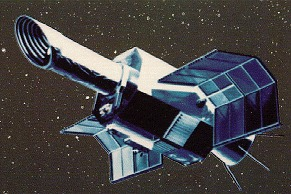
\includegraphics[width=0.30\textwidth]{satellite}
  \end{center}
  \vspace{-20pt}
\end{wrapfigure}
Data di lancio: 26 Gennaio 1978\\
Veicolo di lancio: Delta\\
Sito di lancio: Cape Canaveral, Stati Uniti\\
Massa: 669 Kg\\
Potenza nominale: 424 W\\
Data di disattivazione: 30 Settembre 1996\\

Il progetto è nato da una collaborazione tra NASA, il Science Research Council britannico e l'Agenzia Spaziale Europea (ESA).

L'Ultraviolet Explorer International (IUE) è stato il primo esperimento per esplorare la gamma completa di \textbf{radiazioni ultraviolette} dell'universo, che sono tutte inaccessibili dalla Terra per via dello strato protetttivo di ozono.

L'idea di un satellite dotato di spettrografo ultravioletto venne proposta all'ESRO, il predecessore dell'ESA, da un gruppo di scienziati britannici negli anni '60. Una proposta simile venne avanzata negli Stati Uniti nello stesso periodo da Robert Wilson che lo propose alla NASA. L'ente accolse l'idea del satellite e la sviluppò chiamando il progetto SAS-D (Small Astronomy Satellite-D). Gli scienziati britannici si unirono al progetto e realizzarono la videocamera. ESA si unì al progetto e realizzò i pannelli solari e forni una base a terra. Alla fine il progetto venne rinominato in International Ultraviolet Explorer.

\section*{Osservazioni}
\label{osservazioni}

Le osservazioni di IUE includono praticamente ogni tipo di oggetto dell'universo. Uno dei punti di forza di IUE è stata la capacità di rispondere rapidamente a obiettivi di opportunità, come comete, novae e supernovae.

Il satellite è dotato di un telescopio di 45 centimetri sensibile alla luce ultravioletta. Inoltre, le telecamere spettrografiche a lunghe e corte lunghezze d'onda rilevano la luce ultravioletta da circa 120 a 340 nanometri.

IUE ha ottenuto gli unici dati ultravioletti provenienti dall'esplosione della supernova 1987A nella Grande Nube di Magellano.
Con il monitoraggio del nucleo della cometa IRAS-Araki-Alcock in rapido movimento, IUE è stato in grado di ottenere il primo rilevamento di zolfo molecolare in una cometa.
Nel luglio del 1994 IUE ha trascorso molto tempo ad osservare Giove quando la cometa Shoemaker-Levy era in collisione con esso.
Inoltre, IUE ha rilevato: il fenomeno dell'aurora su Giove, la quantità di acqua persa da una cometa, il forte campo magnetico di particolari stelle, il fenomeno del vento solare su stelle diverse dal sole.

\section*{Curiosità}
\label{curiosit}

Gli astronomi studiano più lunghezze d'onda al fine di conoscere meglio gli oggetti dell'universo. L'acquisizione contemporanea dei dati è essenziale al fine di ottenere il massimo delle conoscenze di alcuni eventi transitori. Così, molto spesso, IUE è stato usato in combinazione con altri telescopi di tutto il mondo.

Secondo l'accordo stipulato tra le agenzie, il tempo utile di osservazione veniva diviso in base al contributo economico fornito dalle agenzie per finanziare il progetto.

Il satellite era posto in un'orbita geosincrona ellittica di periodo un giorno, con apogeo di 42.000 km e perigeo di 26.000 km.

È stato il primo osservatorio spaziale ad operare in tempo reale seguendo gli ordini impartiti dagli astronomi nelle basi a terra in Europa e negli USA.


\end{document}